\documentclass{beamer}

\usepackage[english]{babel}
\usepackage{graphicx,hyperref,ru}
\usepackage{listings}
\usepackage{fancyvrb}
\usepackage{soul}
\usepackage{framed}
\usepackage{xcolor}
\usepackage{gnuplottex}
\lstset{basicstyle=\scriptsize\sffamily}
%\lstset{language=Assembler}[avr8avra] % not standard
\lstdefinestyle{customasm}{
  morekeywords={adc,adiw,asr,brts,brcs,brhs,brne,cbr,clh,clr,clt,cp,cpi,dec,eor,ld,ldi,lpm,lsl,mov,or,rcall,ret,seh,set,st,subi,swap,rjmp,nop},
  morecomment=[l][\color{blue}]{;}
}
\lstset{style=customasm}
%\lstset{basicstyle=\tiny\sffamily}

% A few hacks to get references via bibtex (easy reuse for paper)
\usepackage{bibentry}
\nobibliography*
\let\newblock\relax
\setbeamertemplate{bibliography item}{}

\title[Speed and Size-Optimized PRESENT for AVR]{Speed and Size-Optimized Implementations of the PRESENT Cipher for Tiny AVR Devices}
\author[Papagiannopoulos and Verstegen]{
Kostas Papagiannopoulos \\
Aram Verstegen
}

\date{\today}

\begin{document}
\frame{\titlepage}

\begin{frame}[fragile]
\frametitle{Who We Are}
\includegraphics{ki}
\begin{itemize}
\item 2-year master programme in computer security
\item Collaboration of 3 Universities
\item Software, Hardware, Networks, Formal methods, Cryptography, Privacy, Law, Ethics, Auditing
\item \url{http://kerckhoffs-institute.org/}
\end{itemize}
\end{frame}

\begin{frame}[fragile]
\frametitle{Cryptography Engineering, Assignment 1}
\begin{quote}
``Choose and implement a block cipher on the ATtiny45 in two versions, optimized for size and speed''
\end{quote}

\begin{itemize}
\item PRESENT
\item KATAN-64
\item Klein
\item LED
\item PRINCE
\item mCrypton
\item Piccolo
\item XTEA
\item HIGHT
\end{itemize}
\end{frame}

\begin{frame}[fragile]
\frametitle{ATtiny Platform}
\begin{tabular}{c c c c}
         & Flash ROM (KiloBytes) & SRAM (Bytes) & Clock speed \\
ATtiny25 & 2 & 128 & 20 \\
ATtiny45 & 4 & 256 & 20 \\
ATtiny85 & 8 & 512 & 20 \\
ATtiny1634 & 16 & 1024 & 12 \\
\end{tabular}
\begin{itemize}
\item Basic 90 AVR instructions
\item 32 8-bit general purpose registers
\end{itemize}
\end{frame}

\begin{frame}[fragile]
\frametitle{Quick AVR Recap}
\begin{footnotesize}
\begin{tabular}{l l}
Load register from immediate & \textbf{ldi} \textit{Rd}, \textit{42} \\
Load register from SRAM pointer (X) & \textbf{ld} \textit{Rd}, \textit{X} \\
Load register from ROM pointer (Z) & \textbf{lpm} \textit{Rd}, \textit{Z} \\
XOR output with input & \textbf{eor} \textit{Ro}, \textit{Ri} \\
Swap nibbles in byte & \textbf{swap} \textit{Rd} \\
Rotate left (highest bit goes into carry flag) & \textbf{rol} \textit{Rd} \\
Save to SRAM from register (and increment) & \textbf{st} \textit{X+}, \textit{Rd} \\
Well-known mnemonics & \textbf{and}, \textbf{or}, \textbf{rcall}, \textbf{ret}, \\
                     & \textbf{rjmp}, \textbf{push}, \textbf{pop}, \textbf{inc}, \\
                     & \textbf{dec}, \textbf{add}, \textbf{sub} \\
\end{tabular}
\end{footnotesize}

The 32 general purpose registers are mapped at the start of memory and can be accessed through the \textit{Y} register.
\end{frame}

\begin{frame}[fragile]
\frametitle{Choosing}
\begin{itemize}
\item All 64-bit SPN ciphers with 64 or 80 bit keys
\item None look impossible
\item Some based on matrix multiplication
\end{itemize}
\begin{quote}
``PRESENT looks just about perfect for the hardware and it's only 4
functions, 2 of which are tables and it's XOR based. It's my favorite
so far for sheer simplicity.'' - Aram
\end{quote}

\begin{quote}
``Yep, PRESENT seems straightforward we should definitely opt for it.
We also need a second choice, right? We could go for KATAN, it also looks ok.'' - Kostas
\end{quote}
We got our first choice.
\end{frame}


\begin{frame}[fragile]
\frametitle{PRESENT Cipher}
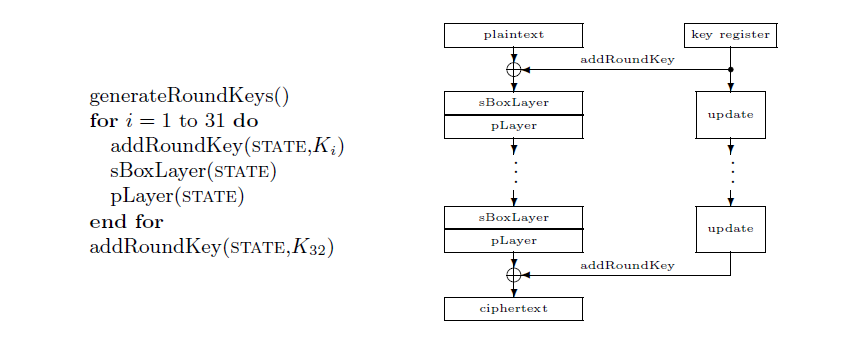
\includegraphics[width=\textwidth]{cipher}
\end{frame}

\begin{frame}[fragile]
\frametitle{Strategy}
\begin{tabular}{c c c }
	& Speed-optimized & Size-optimized \\
Substitution/permutation & Tabled & On-the-fly \\
Code flow & Inlined / unrolled & Re-used / looped \\
Locality & All in registers & Use more SRAM \\
Tricks & Algorithmic & Device-specific \\

\end{tabular}
\end{frame}

\begin{frame}[fragile]
\frametitle{addRoundKey}
\begin{lstlisting}
; state ^= roundkey (first 8 bytes of key register)
addRoundKey:
    eor STATE0, KEY0
    eor STATE1, KEY1
    eor STATE2, KEY2
    eor STATE3, KEY3
    eor STATE4, KEY4
    eor STATE5, KEY5
    eor STATE6, KEY6
    eor STATE7, KEY7
    ret
\end{lstlisting}
\end{frame}

\begin{frame}[fragile]
\frametitle{4-bit S-Box}
	\begin{tabular}{ | c | c | c | c | c | c | c | c | c | c | c | c | c | c | c | c | c | }
	  \hline                        
	     x & 0 & 1 & 2 & 3 & 4 & 5 & 6 & 7 & 8 & 9 & A & B & C & D & E & F \\
	  \hline                        
	  S[x] & C & 5 & 6 & B & 9 & 0 & A & D & 3 & E & F & 8 & 4 & 7 & 1 & 2 \\
	  \hline  
	\end{tabular}

\begin{itemize}
\item Original:
  \begin{lstlisting}
  .db 0x0C, 0x05, 0x06, 0x0B ...
  \end{lstlisting}
\item Compact:
  \begin{lstlisting}
  .db 0xC5, 0x6B, 0x90, 0xAD ...
  \end{lstlisting}
\item Accessing the table 4 bits at a time incurs a penalty
\item Cost to substitutes a byte: two clearings of nibbles, two lookups, two settings of nibbles, two swapping of nibbles
\item We have an 8-bit architecture, so we want to access bytes!
\end{itemize}
\end{frame}

\begin{frame}
\frametitle{Squared S-Box}
\begin{tabular}{| c | c  | c | c | c  | c  | c | c | c  | c | c | c |}
\hline
  x & 00 & 01 & 02 & 03  &  $\dots$  & 0C & 0D & 0E & 0F   \\
\hline
 S[x] & CC & C5 & C6 & CB & \dots & C4 & C7 & C1 & C2   \\
\hline
  x & 10 & 11 & 12 & 13  &  $\dots$  & 1C & 1D & 1E & 1F   \\
\hline
 S[x] & 5C & 55 & 56 & 5B & \dots & 54 & 57 & 51 & 52   \\
\hline
  \vdots & \vdots & \vdots & \vdots & \vdots  &  $\dots$  & \vdots &\vdots & \vdots & \vdots   \\
\hline
  x & F0 & F1 & F2 & F3  &  $\dots$  & FC & FD & FE & FF   \\
\hline
 S[x] & 2C & 25 & 26 & 2B & \dots & 24 & 27 & 21 & 22   \\
\hline
\end{tabular}

\begin{itemize}
\item New S-Box is 256 bytes, $16\cdot16$ combinations of 4-bits
\item It substitutes 1 byte at a time
\item No need to swap or discern high/low byte part
\item Cost to substitute a byte: only 1 lookup
\end{itemize}
\end{frame}

\begin{frame}[fragile]
\frametitle{S-Box and P-Layer}
%\begin{itemize}
%\item
\emph{Idea: Combine the SBox and PLayer in lookup tables} [Bo Zhu \& Zheng Gong]
%\end{itemize}
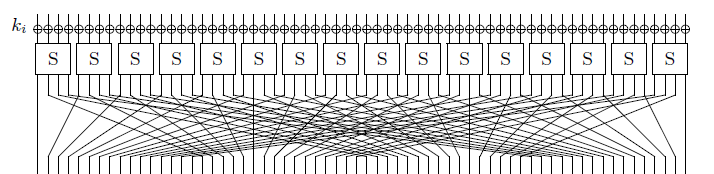
\includegraphics[width=\textwidth]{spnet.png}
\begin{itemize}
\item 1024 bytes of lookup tables, 32 lookups per round
\item Works well on AVR compared to on-the-fly calculation
  \begin{itemize}
    \item Reached \emph{8700cc} for encryption
  \end{itemize}
\item Because of many lookups, consider larger SRAM
  \begin{itemize}
    \item \textit{lpm} instruction: 3cc
    \item \textit{ld} instruction: 2cc, could reduce ~2000cc more
  \end{itemize}
\end{itemize}
\end{frame}

\begin{frame}[fragile]
\frametitle{Lookup tables}
\begin{minipage}[t]{0.48\textwidth}

\begin{itemize}
\item Table 1 at \textit{0x600}, Table 2 at \textit{0x800}
\item Lookup table 1
\begin{lstlisting}
    ldi ZH, 0x06
    mov ZL, STATE0
    lpm OUTPUT0, Z
\end{lstlisting}
\item Lookup table 2
\begin{lstlisting}
    ldi ZH, 0x08
    mov ZL, STATE1
    lpm OUTPUT1, Z
\end{lstlisting}
\end{itemize}
\end{minipage}
\hfill
\begin{minipage}[t]{0.48\textwidth}
\begin{itemize}
\item \st{Lookup table 1, table 2, table 1, table 2}
\item Lookup table 1, table 1, table 2, table 2
\begin{lstlisting}
    ldi ZH, 0x06
    mov ZL, STATE0
    lpm OUTPUT0, Z
    mov ZL, STATE2
    lpm OUTPUT2, Z

    ldi ZH, 0x08
    mov ZL, STATE1
    lpm OUTPUT1, Z
    mov ZL, STATE3
    lpm OUTPUT3, Z
\end{lstlisting}
\item Fewer changes in \textit{ZH}
\end{itemize}
\end{minipage}
\end{frame}

\begin{frame}
\frametitle{Key Update}
\begin{enumerate}
\item Rotate 80-bit key register 61 bits to the left
  \begin{itemize}
  \item Rotate 19 bits to the right in stead
  \item Use 2 \textit{mov} instructions to rotate $2\cdot8=16$ bits
  \item Use \textit{ror} only for the last 3 bits
  \end{itemize}
\item S-Box the top 4 bits of 80-bit key register
  \begin{itemize}
  \item Use a \textbf{byte} lookup table
  \end{itemize}
\item XOR key bits with round counter
  \begin{itemize}
  \item XOR needs to span 2 registers
  \item Do step 3 before step 1 then XOR spans only 1 register
  \end{itemize}
\end{enumerate}
\end{frame}

\begin{frame}
\frametitle{AVR Architecture}
        \begin{itemize}
        \item 16-bit opcodes
        \item Harvard architecture
        \item No bulk instructions
        \item Some SRAM
        \item SREG flags
        \item SWAP instruction
        \item CBR instruction
        \item All kinds of branching instructions
        \end{itemize}
\end{frame}

\begin{frame}
\frametitle{Optimization Strategy}
        \begin{itemize}
        \item Be concise to start with
        \item Look for repeating patterns
        \item Refactor to reuse code wherever possible
        \item Use the SRAM more
        \item Employ a different I/O pattern
        \end{itemize}
\end{frame}

\begin{frame}[fragile]
\frametitle{Serialization of the Algorithm}
\begin{lstlisting}
; state ^= roundkey
addRoundKey:
    eor STATE0, KEY0
    eor STATE1, KEY1
    eor STATE2, KEY2
    eor STATE3, KEY3
    eor STATE4, KEY4
    eor STATE5, KEY5
    eor STATE6, KEY6
    eor STATE7, KEY7
    ret
\end{lstlisting}
\end{frame}

\begin{frame}[fragile]
\frametitle{Serialization of the Algorithm}
\begin{minipage}[t]{0.48\textwidth}
\begin{lstlisting}
; half state ^= roundkey
addRoundKey:
    eor STATE0, KEY0
    eor STATE1, KEY1
    eor STATE2, KEY2
    eor STATE3, KEY3
    ret
\end{lstlisting}

This helps with:
\begin{itemize}
        \item doing I/O
        \item applying round keys
        \item applying S-Boxes
        \item applying P-layer
\end{itemize}
\end{minipage}
\hfill
\begin{minipage}[t]{0.48\textwidth}
But we need I/O:
\begin{lstlisting}
consecutive_input:
    ld STATE0, X+
    ld STATE1, X+
    ld STATE2, X+
    ld STATE3, X+
    ret

interleaved_output:
    st STATE3, X-
    dec X
    st STATE2, X-
    dec X
    st STATE1, X-
    dec X
    st STATE0, X-
    dec X
    ret
\end{lstlisting}
And we need to rotate the key register
\end{minipage}
\end{frame}

\begin{frame}[fragile]
\frametitle{Indirect Register Access}
\begin{lstlisting}
; state ^= roundkey (full state in SRAM)
addRoundKey:
      clr YL               ; point Y at first key register
addRoundKey_byte:
      ld ITEMP, X          ; load input
      ld KEY_BYTE, Y+      ; load key, advance pointer
      eor ITEMP, KEY_BYTE  ; XOR
      st X+, ITEMP         ; store output, advance pointer

      cpi YL, 8            ; loop over 8 bytes
      brne addRoundKey_byte

      subi XL, 8           ; point at the start of the block
      ret
\end{lstlisting}
\end{frame}

\begin{frame}[fragile]
\frametitle{Packing S-Boxes}
	\footnotesize{
	Before: \\
	\begin{tabular}{ | c | c | c | c | c | c | c | c | c | c | c | c | c | c | c | c | }
	  \hline                        
	  C & 5 & 6 & B & 9 & 0 & A & D & 3 & E & F & 8 & 4 & 7 & 1 & 2 \\
	  \hline  
	\end{tabular}
	\\

	After: \\
	\begin{tabular}{ | c | c | c | c | c | c | c | c | }
	  \hline                        
	  C5 & 6B & 90 & AD & 3E & F8 & 47 & 12 \\
	  \hline  
	\end{tabular}
	}

\begin{lstlisting}
unpack_sBox:
    asr ZL                ; halve input, take carry
    lpm SBOX_OUTPUT, Z    ; get s-box output
    brcs odd_unpack       ; branch depending on carry
even_unpack:
    swap SBOX_OUTPUT      ; swap nibbles in s-box output
odd_unpack:
    cbr SBOX_OUTPUT, 0xf0 ; clear high nibble in s-box output
    ret
\end{lstlisting}
\begin{verbatim}




\end{verbatim}
\end{frame}

\begin{frame}[fragile]
\frametitle{Packing S-Boxes and unpacking in constant time}
	\footnotesize{
	Before: \\
	\begin{tabular}{ | c | c | c | c | c | c | c | c | c | c | c | c | c | c | c | c | }
	  \hline                        
	  C & 5 & 6 & B & 9 & 0 & A & D & 3 & E & F & 8 & 4 & 7 & 1 & 2 \\
	  \hline  
	\end{tabular}
	\\

	After: \\
	\begin{tabular}{ | c | c | c | c | c | c | c | c | }
	  \hline                        
	  C5 & 6B & 90 & AD & 3E & F8 & 47 & 12 \\
	  \hline  
	\end{tabular}
	}

\begin{lstlisting}
unpack_sBox:
    asr ZL
    lpm SBOX_OUTPUT, Z
    brcs odd_unpack       ; 2 cycles if true
even_unpack:
    swap SBOX_OUTPUT      ; 1 cycle
    rjmp unpack           ; 2 cycles
odd_unpack:
    nop                   ; 1 cycle
    nop
; 4 cycles total
unpack:
    cbr SBOX_OUTPUT, 0xf0
    ret
\end{lstlisting}
\end{frame}

\begin{frame}[fragile]
\frametitle{S-Box Optimization}
\begin{lstlisting}
sBoxByte:
    ; input (low nibble)
    mov ZL, ITEMP         ; load s-box input
    cbr ZL, 0xf0          ; clear high nibble in input
    rcall unpack_sBox     ; get output in SBOX_OUTPUT

    cbr ITEMP, 0xf        ; clear low nibble in output
    or ITEMP, SBOX_OUTPUT ; save low nibble to output

    ; fall through
sBoxHighNibble:
    mov ZL, ITEMP         ; load s-box input
    cbr ZL, 0xf           ; clear low nibble in input
    swap ZL               ; move high nibble to low nibble

    rcall unpack_sBox     ; get output in SBOX_OUTPUT
    swap SBOX_OUTPUT      ; move low nibble to high nibble

    cbr ITEMP, 0xf0       ; clear high nibble in output
    or ITEMP, SBOX_OUTPUT ; save high nibble to output

    ret
\end{lstlisting}
\end{frame}

\begin{frame}[fragile]
\frametitle{S-Box Optimization}
\begin{lstlisting}
sBoxByte:
    rcall sBoxLowNibbleAndSwap ; apply s-box to low nibble
                               ; and swap nibbles
    rjmp sBoxLowNibbleAndSwap  ; do it again and return
sBoxHighNibble:
    swap ITEMP                 ; swap nibbles in IO register
sBoxLowNibbleAndSwap:
    mov ZL, ITEMP              ; load s-box input
    cbr ZL, 0xf0               ; clear high nibble in s-box input

    rcall unpack_sBox

    cbr ITEMP, 0xf             ; clear low nibble in IO register
    or ITEMP, SBOX_OUTPUT      ; save low nibble to IO register
    swap ITEMP                 ; swap nibbles
    ret
\end{lstlisting}
\end{frame}

\begin{frame}[fragile]
\frametitle{S-Box Optimization}
\begin{lstlisting}
sBoxByte:
    rcall sBoxLowNibbleAndSwap ; apply s-box to low nibble
                               ; and swap nibbles
    rjmp sBoxLowNibbleAndSwap  ; do it again and return
sBoxHighNibble:
    swap ITEMP                 ; swap nibbles in IO register
sBoxLowNibbleAndSwap:
    mov ZL, ITEMP              ; load s-box input
    cbr ZL, 0xf0               ; clear high nibble in s-box input

unpack_sBox:
    asr ZL                     ; halve input, take carry
    lpm SBOX_OUTPUT, Z         ; get s-box output
    brcs odd_unpack            ; branch depending on carry
even_unpack:
    swap SBOX_OUTPUT           ; swap nibbles in s-box output
odd_unpack:
    cbr SBOX_OUTPUT, 0xf0      ; clear high nibble in s-box output

    cbr ITEMP, 0xf             ; clear low nibble in IO register
    or ITEMP, SBOX_OUTPUT      ; save low nibble to IO register
    swap ITEMP                 ; swap nibbles
    ret
\end{lstlisting}
\end{frame}

%\begin{frame}[fragile]
%\frametitle{Size Over Time}
%%\includegraphics[width=\textwidth]{size_over_time}
%\tiny{
%\advance\leftskip-4em
%\begin{gnuplot}[terminal=latex]
%set xdata time
%set timefmt "%b-%d"
%set xrange ["Feb-23":"Mar-4"]
%set yrange [250:500]
%set xlabel "Time"
%set ylabel "Size"
%set title "Size reduction of my PRESENT implementation"
%set key off
%set output "size_over_time_february.tex"
%plot "size_over_time_february.txt" using 1:2 index 0 title "bytes" with points, \
     %''               using 1:2:2 with labels left offset 0.8,0.2 notitle, \
     %''               using 1:2:3 with labels left offset 3,0.2 notitle

%\end{gnuplot}
%\include{size_over_time_february}
%}
%\end{frame}

\begin{frame}[fragile]
\frametitle{Using SREG Flags}
\begin{lstlisting}
setup_redo_block:
        clt                   ; clear T flag
        rjmp redo_block       ; do the second part
block:
        set                   ; set T flag
        ; fall through
redo_block:
        ; instructions here happen twice when called from block

        brts setup_redo_block ; redo this block? (if T flag set)
        ret
\end{lstlisting}
\end{frame}


%\begin{frame}[fragile]
%\frametitle{Size Over Time}
%%\includegraphics[width=\textwidth]{size_over_time}
%\tiny{
%\advance\leftskip-4em
%\begin{gnuplot}[terminal=latex]
%set xdata time
%set timefmt "%b-%d"
%set xrange ["May-20":"Jul-1"]
%set yrange [250:500]
%set xlabel "Time"
%set ylabel "Size"
%set title "Size reduction of my PRESENT implementation"
%set key off
%set output "size_over_time_june.tex"
%plot "size_over_time_june.txt" using 1:2 index 0 title "bytes" with points, \
     %''               using 1:2:2 with labels left offset 0.8,0.2 notitle, \
     %''               using 1:2:3 with labels left offset 3,0.2 notitle

%\end{gnuplot}
%\include{size_over_time_june}
%}
%\end{frame}

\begin{frame}[fragile]
\frametitle{Size Per Procedure}
%\includegraphics[width=\textwidth]{procedures}
\tiny{
\advance\leftskip-4em
\begin{gnuplot}[terminal=latex]
set yrange [0:65]
set xlabel "Procedure"
set ylabel "Size"
set title "Sizes per procedure"
set key left box
unset xtics
set output "procedures.tex"
plot 'procedures.txt' using 0:2:xtic(1) title "bytes" with boxes, \
     ''          using 0:2:1 with labels offset 0,0.5 notitle
\end{gnuplot}
\include{procedures}
}
\end{frame}

\begin{frame}[fragile]
\frametitle{Numbers}
\begin{table}[h]
\centering
\footnotesize
	\begin{tabular}{ l r r r }
		& Encryption & Decryption & Size \\
	\textbf{Papagiannopoulos} & 8721 & - & 1794 \\
	AVR Crypto-lib & 105796 & 151624 & 1514 \\
	Eisenbarth & 10723 & 11239 & 936 \\
	\textbf{Verstegen} & & & \\
	\hspace{0.4em} Inlined rotation, unpacked S-Boxes (128-bit) &  64506 & 119626 & 292 \\
	\hspace{0.4em} Inlined rotation (128-bit)                   &  67854 & 123346 & 290 \\
	\hspace{0.4em} Inlined rotation, unpacked S-Boxes           &  52622 &  73952 & 280 \\
	\hspace{0.4em} Inlined rotation                             &  55784 &  77300 & 278 \\
	\hspace{0.4em} Unpacked S-Boxes                             & 186883 & 250032 & 274 \\
	\hspace{0.4em} Unpacked S-Boxes (128-bit)                   & 278189 & 568010 & 274 \\
	\hspace{0.4em} Default                                      & 190045 & 253380 & 272 \\
	\hspace{0.4em} Default (128-bit)                            & 281537 & 571730 & 272 \\
	\end{tabular}
	\label{numbers}

\end{table}
\end{frame}

\begin{frame}[fragile]
\frametitle{Relative Performance/Size}
\tiny{
\advance\leftskip-4em
\begin{gnuplot}[terminal=latex]
set terminal latex
set output "cycles_byte.tex"
set yrange [200:1900]
set xlabel "Cycles/byte"
set ylabel "Size"
set title "Efficiency vs Size"
plot "cycles_byte.txt" notitle with points, \
     ''               using 1:2:3 with labels left offset 1,0 notitle

\end{gnuplot}
\include{cycles_byte}
}
\end{frame}

\begin{frame}[fragile]
\frametitle{Binary QR Code}
\includegraphics[width=0.5\textwidth]{qr2}
%\includegraphics[width=0.5\textwidth]{qr3}

\textbf{Not} a URL - may crash QR apps
\end{frame}

\begin{frame}[fragile]
\frametitle{ASCII Art}
\scriptsize{
%\begin{snugshade}
    \begin{Verbatim}[commandchars=\\\{\}]
C56B90AD   3EF84712   5EF8C12    DB4630  79A57D0  3AD0    F1F  7F0E070E1
41D05DD05  CD047D080  2D16D00   82E81E1  06D0542  682E0   03D  04A9591F7
33C0CAE08  894CA9598  81991F9   883CD13  FACF9D1  E8A95   A9F  7089504D0
829   502  D08   295  089       5E8      2FE      F70E70  FE5     955
491  10F0  529   502  C00       0000     000      5F7080  7F8     52B
089587950  795879517  9587952   795879   5379508  9543958 6E0     D5D
F442687E3  D2DF802DD  DDF082E   4F31089  5CC278C  916 991 862     78D
93C830D1   F7A85008   9568E08     C91CD  DF8D936  A95 D9F7A85     008
954        427 F0E0   70E          0189  6DD      27C  C278D9     189
93C        A30 E1F7A  251      08   956  894      189  664E08     E91
CAD        FC9  DF6A  95D9F73  F932F931  F930F93  16F   4E894     F3C
F68        941   7966 4E08F91  8E93AA95  6A95D9F  71E   F4E89     419
96F        6CF   0895D7DFC5DF  CDDFE0D   FB7DFD9  F7C    0CF0     000
    \end{Verbatim}
%\end{snugshade}
}
\end{frame}

\begin{frame}[fragile]
\frametitle{ASCII Art}
\scriptsize{
%\begin{snugshade}
    \begin{Verbatim}[commandchars=\\\{\}]
s-boxes                                     decrypt (start+16)
|                                           |
\textcolor{black}{C56B90AD   3EF84712   5EF8C12    DB4630  79A}\textcolor{red}{57D0  3AD0    F1F  7F0E070E1}
\textcolor{red}{41D05DD05  CD047D080  2D16D00   82E81E1  06D0542  682E0   03D  04A9591F7}
\textcolor{red}{33C0}\textcolor{orange}{CAE08  894CA9598  81991F9   883CD13  FACF9D1  E8A95   A9F  70895}\textcolor{blue}{04D0}
\textcolor{blue}{829   502  D08   295  089       5}\textcolor{purple}{E8      2FE      F70E70  FE5     955}
\textcolor{purple}{491  10F0  529   502  C00       0000     000      5F7080  7F8     52B}
\textcolor{purple}{0895}\textcolor{brown}{87950  795879517  9587952   795879   5379508  95}\textcolor{cyan}{43958 6E0     D5D}
\textcolor{cyan}{F442687E3  D2DF802DD  DDF082E   4F31089  5}\textcolor{red}{CC278C  916 991 862     78D}
\textcolor{red}{93C830D1   F7A85008   95}\textcolor{magenta}{68E08     C91CD  DF8D936  A95 D9F7A85     008}
\textcolor{magenta}{95}\textcolor{pink}{4        427 F0E0   70E          0189  6DD      27C  C278D9     189}
\textcolor{pink}{93C        A30 E1F7A  251      08   95}\textcolor{yellow}{6  894      189  664E08     E91}
\textcolor{yellow}{CAD        FC9  DF6A  95D9F73  F932F931  F930F93  16F   4E894     F3C}
\textcolor{yellow}{F68        941   7966 4E08F91  8E93AA95  6A95D9F  71E   F4E89     419}
\textcolor{yellow}{96F        6CF   0895}\textcolor{green}{D7DFC5DF  CDDFE0D   FB7DFD9  F7C    0CF0     000}
                     |
                     encrypt (end-16)

    S-Boxes, \textcolor{red}{decrypt}, \textcolor{orange}{rotate_left_i}, \textcolor{blue}{sBoxByte}, \textcolor{purple}{sBoxNibble}, \textcolor{brown}{pLayerNibble},
    \textcolor{cyan}{schedule_key}, \textcolor{red}{addRoundKey}, \textcolor{magenta}{sBoxLayer}, \textcolor{pink}{setup}, \textcolor{yellow}{pLayer}, \textcolor{green}{encrypt}.
    \end{Verbatim}
%\end{snugshade}
}
\end{frame}

\begin{frame}[fragile]
\frametitle{Questions?}
	\footnotesize{
	\url{https://github.com/aczid/ru_crypto_engineering/}
	\url{https://github.com/kostaspap88/PRESENT_speed_implementation/}
	}
	
\includegraphics[width=0.5\textwidth]{qr_url}
	
\includegraphics[width=0.5\textwidth]{qr_url2}
\end{frame}

\end{document}
